\scanpage{84}
% archive foliation: 83
\uline{IV}\quad \unsure{4.1.2}\quad
4.1.2 \unsure{trivial} in terms of \uline{III} p. 16 added.

Quite \inserted{\unsure{for $s^*$}} cumbersome; take point of
$\operatorname{Spec}(\underline O_{S,s})$!

6\quad Introduce geometric points of $S$.

\uline{VI}\quad 2\quad\unsure{inutile}

7\quad What is the meaning?

$\left.\begin{array}{l}9\\11\end{array}\right\}$
6.1.1 and 6.2.2 could be made into a single example!

\margin{\figure{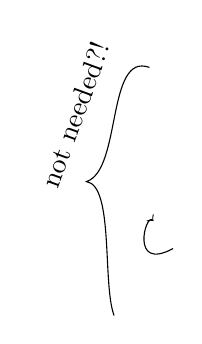
\begin{tikzpicture}[x=1cm,y=1cm]
\draw (1,3.4) .. controls (.45,3.6) and (.65,2.1) .. (.20,1.95) .. controls (.55,1.90) and (.40,.65) .. (.55,.25);
\node[rotate=70] at (.05,2.8) {not needed?!};
\draw[->] (1.3,1.1) .. controls (.75,.8) and (.95,1.55) .. (1.05,1.45);
\end{tikzpicture}}}

VII\quad 1

2\quad I guess that one has equivalence of categories anyhow!!

\margin{\figure{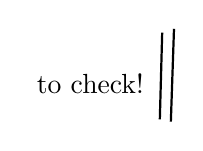
\begin{tikzpicture}[x=1cm,y=1cm]
\node[anchor=east] at (0,.45) {to check!};
\draw[line width=.8pt] (.08,0)--(.11,1.1) (.22,-.03)--(.26,1.15);
\end{tikzpicture}}}

9

\uline{VIII}\quad 1\\
\hspace*{3em}2

$3/\unsure{8.1.6|8.1.1}$ Not too clear. Say that if
\deleted{$A$ a local or \deleted{\unsure{local}} henselian ring, then to any}
\inserted{$S$ any scheme}
(for instance the localization of $S$ at $s_0$)
and \deleted{$s_0,s_0^*$ two points,}
$x,y$ two points, $x\in\overline{\{y\}}$,
\deleted{then the} with, given just geom. $\bar x,\bar y$
$\overline{k(x)}/x$, $\overline{k(y)}/y$, then the ``paths'' of $\bar y$ to $\bar x$
\deleted{$\unsure{\bar x},\bar y$}
correspond exactly to the \deleted{point} liftings
i.e. to the \inserted{$k(y)$-}hom of
\[
\operatorname{ring}(\overline S\otimes_S y)=\prod K_i
\quad\text{into }\overline{k(y)}.
\]
\diagram{
\begin{tikzcd}
{\overline S=\text{strict loc. of $S$ at $\bar x$}}\arrow[d]
& \bar y^{\unsure{\prime}}\arrow[l,dashed]\arrow[dl]\\
S&
\end{tikzcd}
}

\uuline{IX}\quad
$\begin{array}{ll}
1&14\ \deleted{\unsure{et}}\\
4&\\
5,6&\\
9&\\
10'&18\\
10''&19\\
12&
\end{array}$

$9.3.4\Rightarrow9.3.5$\quad looks tautological

$9.3.5\Rightarrow9.3.2$\quad very cumbersome!

\margin{yoga \unsure{stemming} from Abhyankar lemma to be used...}
